\input{../../tikz-header.tex}
\usepackage{mhchem}
\usepackage{hyperref}

\begin{document}
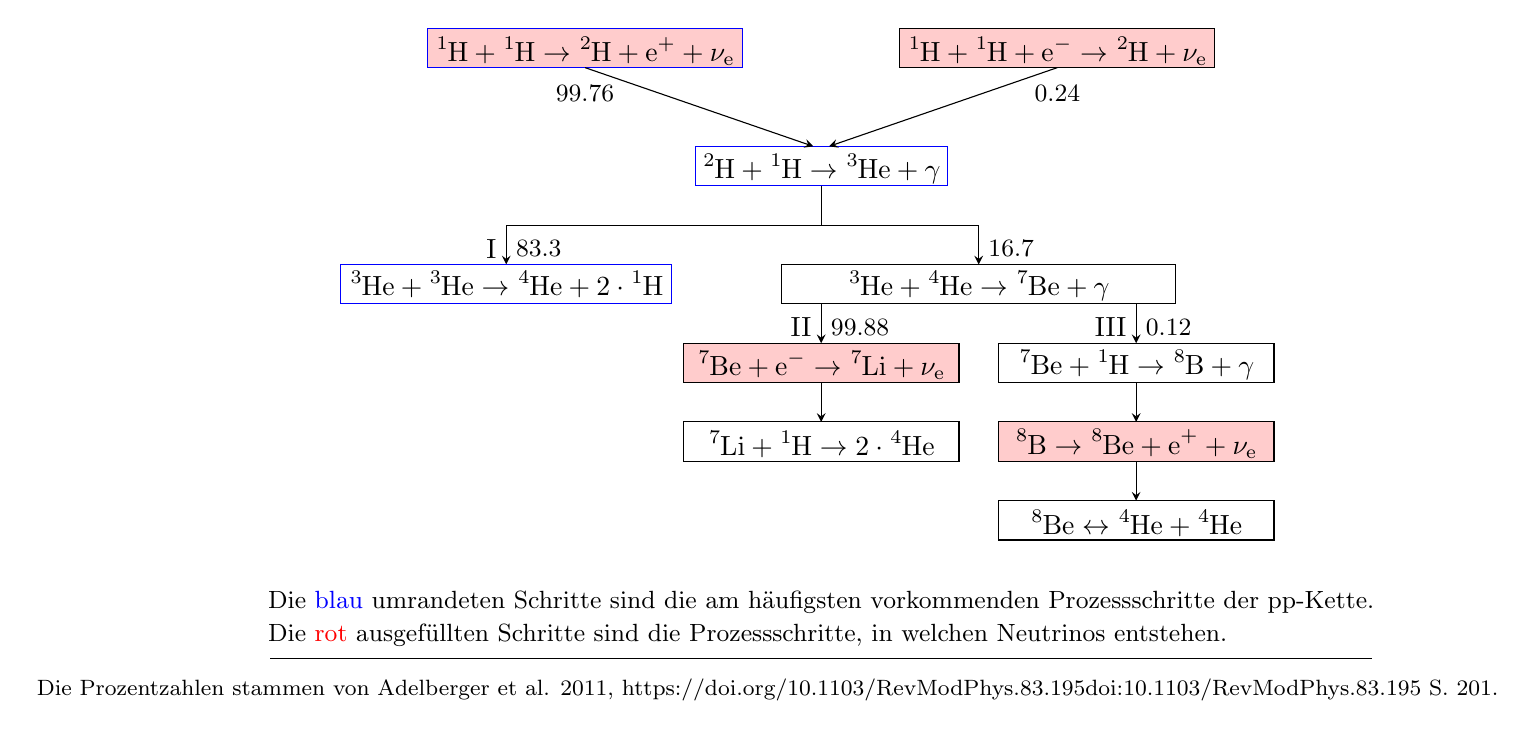
\begin{tikzpicture}
    \draw[blue, fill=red, fill opacity=0.2] (-5,0) rectangle (-1,-0.5);
    \node[above, yshift=-0.1cm] at (-3, -0.5) {$\ce{^1H} + \ce{^1H} \to \ce{^2H} + \ce{e+} + \nu_{\ce{e}}$};

    \draw[fill=red, fill opacity=0.2] (5,0) rectangle (1,-0.5);
    \node[above, yshift=-0.1cm] at (3, -0.5) {$\ce{^1H} + \ce{^1H} + \ce{e-} \to \ce{^2H} + \nu_{\ce{e}}$};

    \draw[blue] (-1.6,-1.5) rectangle (1.6,-2);
    \node[above, yshift=-0.1cm] at (0, -2) {$\ce{^2H} + \ce{^1H} \to \ce{^3He} + \gamma$};

    \draw[->, >=stealth] (3, -0.5) node[below, yshift=-0.1cm]{\small{$\SI{0.24}{\percent}$}} -- (0.1, -1.5);
    \draw[->, >=stealth] (-3, -0.5) node[below, yshift=-0.1cm]{\small{$\SI{99.76}{\percent}$}} -- (-0.1, -1.5);

    \draw (0,-2) -- (0, -2.5);
    \draw (-4,-2.5) -- (2, -2.5);

    % branch I

    \draw[->, >=stealth] (-4,-2.5) -- (-4,-3) node[right, yshift=0.2cm]{\small{$\SI{83.3}{\percent}$}} node[left, yshift=0.2cm]{I};
    \draw[blue] (-6.1,-3) rectangle (-1.9,-3.5);
    \node[above, yshift=-0.05cm] at (-4, -3.5) {$\ce{^3He} + \ce{^3He} \to \ce{^4He} + 2\cdot\ce{^1H}$};

    % branch II & III

    \draw[->, >=stealth] (2,-2.5) -- (2,-3) node[right, yshift=0.2cm]{\small{$\SI{16.7}{\percent}$}};

    \draw (-0.5,-3) rectangle (4.5,-3.5);
    \node[above, yshift=-0.085cm] at (2, -3.5) {$\ce{^3He} + \ce{^4He} \to \ce{^7Be} + \gamma$};

    % branch II

    \draw[->, >=stealth] (0,-3.5) -- (0,-4) node[right, yshift=0.2cm]{\small{$\SI{99.88}{\percent}$}} node[left, yshift=0.2cm]{II};

    \draw[fill=red, fill opacity=0.2] (-1.75,-4) rectangle (1.75,-4.5);
    \node[above, yshift=-0.085cm] at (0, -4.5) {$\ce{^7Be} + \ce{e-} \to \ce{^7Li} + \nu_{\ce{e}}$};

    \draw[->, >=stealth] (0,-4.5) -- (0,-5);

    \draw (-1.75,-5) rectangle (1.75,-5.5);
    \node[above, yshift=-0.085cm] at (0, -5.5) {$\ce{^7Li} + \ce{^1H} \to 2\cdot\ce{^4He}$};

    % branch III

    \draw[->, >=stealth] (4,-3.5) -- (4,-4) node[right, yshift=0.2cm]{\small{$\SI{0.12}{\percent}$}} node[left, yshift=0.2cm]{III};

    \draw (2.25,-4) rectangle (5.75,-4.5);
    \node[above, yshift=-0.085cm] at (4, -4.5) {$\ce{^7Be} + \ce{^1H} \to \ce{^8B} + \gamma$};

    \draw[->, >=stealth] (4,-4.5) -- (4,-5);

    \draw[fill=red, fill opacity=0.2] (2.25,-5) rectangle (5.75,-5.5);
    \node[above, yshift=-0.085cm] at (4, -5.5) {$\ce{^8B} \to \ce{^8Be} + \ce{e+} + \nu_{\ce{e}}$};

    \draw[->, >=stealth] (4,-5.5) -- (4,-6);

    \draw (2.25,-6) rectangle (5.75,-6.5);
    \node[above, yshift=-0.085cm] at (4, -6.5) {$\ce{^8Be} \leftrightarrow \ce{^4He} + \ce{^4He}$};


    \node[align=left] at (0,-7.5) {\small{Die {\color{blue}blau} umrandeten Schritte sind die am häufigsten vorkommenden Prozessschritte der pp-Kette.}\\ \small{Die {\color{red}rot} ausgefüllten Schritte sind die Prozessschritte, in welchen Neutrinos entstehen.}};


    \draw (-7,-8) -- (7,-8);
    \node[align=left, yshift=0.1cm, xshift=-0.68cm] at (0,-8.5){\footnotesize{Die Prozentzahlen stammen von Adelberger et al. 2011, \href{https://doi.org/10.1103/RevModPhys.83.195}{doi:10.1103/RevModPhys.83.195} S. 201.}};

\end{tikzpicture}
\end{document}